\documentclass{article}
\usepackage{tikz}
\usetikzlibrary{positioning}

\begin{document}
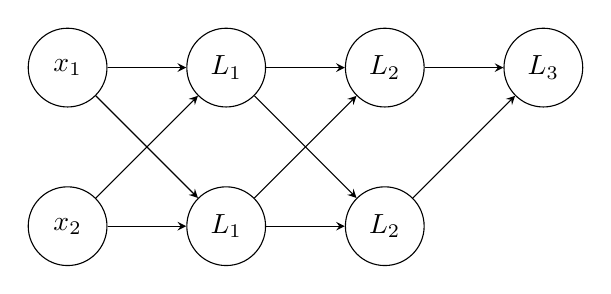
\begin{tikzpicture}[%
    input/.style={%
        draw,
        circle,
        inner sep=2pt,
        minimum size=1cm,
        node distance=1cm
    },
    hidden/.style={%
        draw,
        circle,
        inner sep=2pt,
        minimum size=1cm,
        node distance=1cm
    },
    output/.style={%
        draw,
        circle,
        inner sep=2pt,
        minimum size=1cm,
        node distance=1cm
    },
    >=stealth
]

% Input layer
\node[input] (input1) {$x_1$};
\node[input, below=of input1] (input2) {$x_2$};

% Hidden layer 1 (L_1)
\node[hidden, right=of input1] (hidden1) {$L_1$};
\node[hidden, below=of hidden1] (hidden2) {$L_1$};

% Hidden layer 2 (L_2)
\node[hidden, right=of hidden1] (hidden3) {$L_2$};
\node[hidden, below=of hidden3] (hidden4) {$L_2$};

% Output layer (L_3)
\node[output, right=of hidden3] (output1) {$L_3$};

% Arrows
\draw[->] (input1) -- (hidden1);
\draw[->] (input1) -- (hidden2);
\draw[->] (input2) -- (hidden1);
\draw[->] (input2) -- (hidden2);

\draw[->] (hidden1) -- (hidden3);
\draw[->] (hidden1) -- (hidden4);
\draw[->] (hidden2) -- (hidden3);
\draw[->] (hidden2) -- (hidden4);

\draw[->] (hidden3) -- (output1);
\draw[->] (hidden4) -- (output1);

\end{tikzpicture}
\end{document}
